\begin{figure}[t]
    \centering
    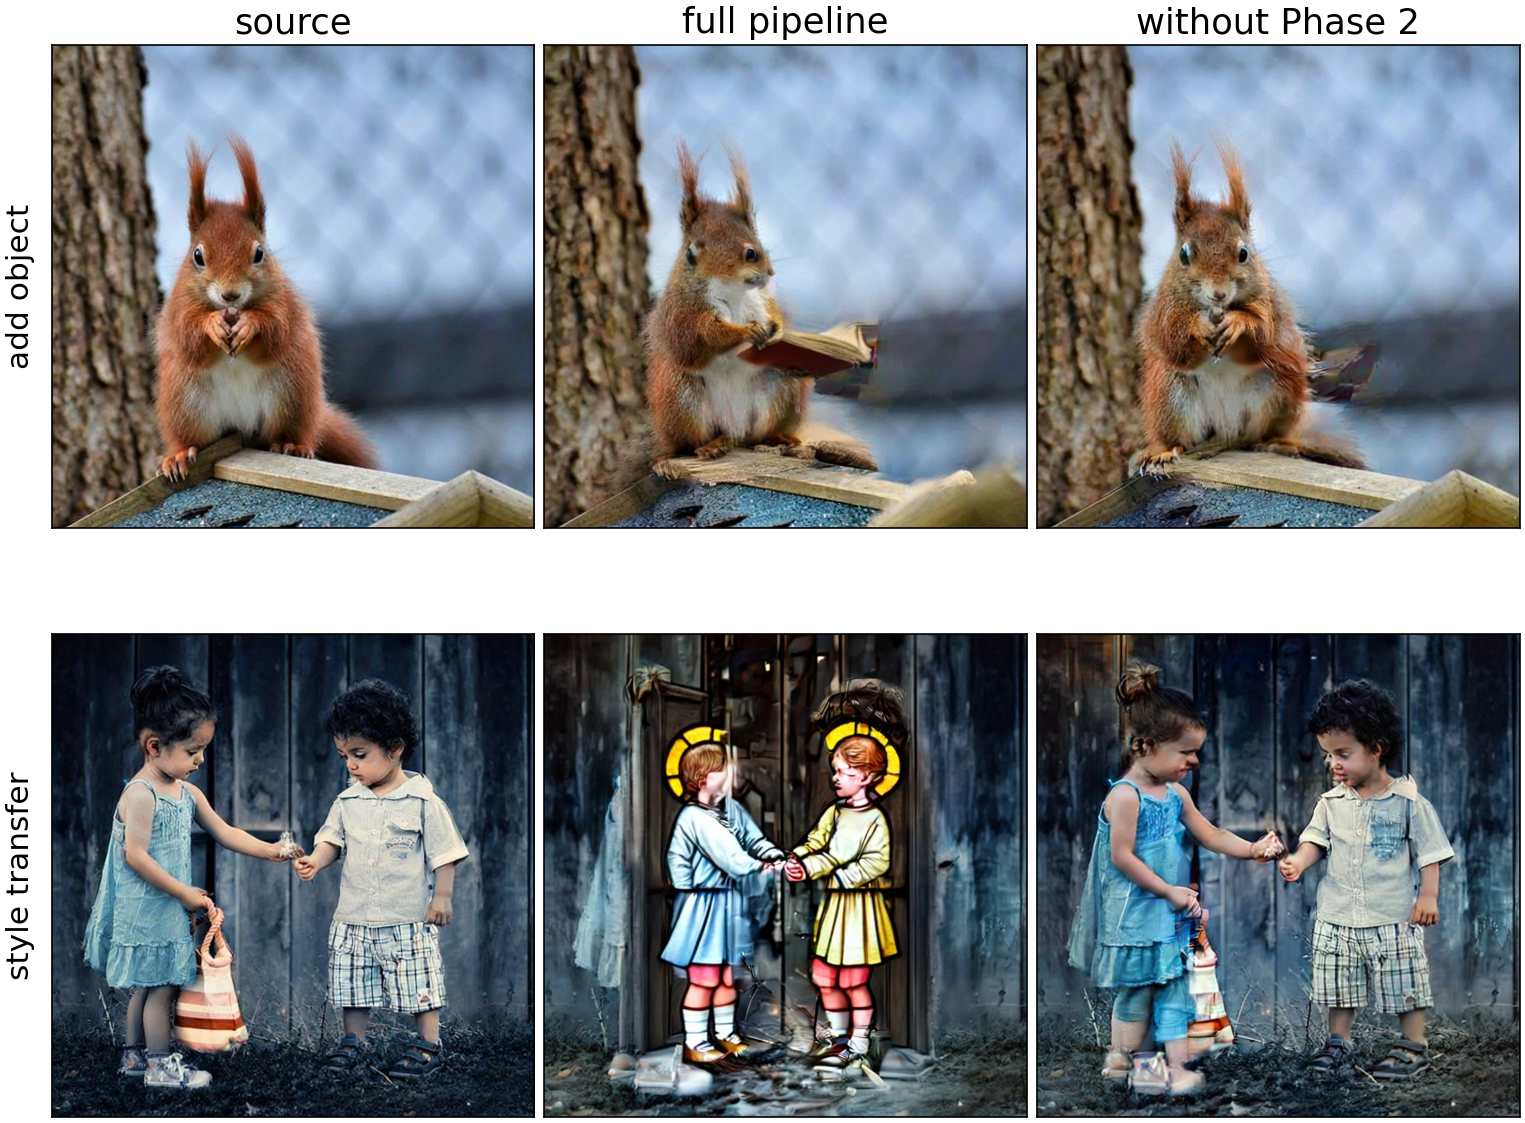
\includegraphics[width=\linewidth]{imgs/fig_beta_qualitative.png}
    \caption{Why Phase~2 is needed. \textbf{Top:} object addition. Without a target-side mask the free-generation region is the source focus alone, so the book has nowhere to grow and the output is nearly the source. \textbf{Bottom:} style transfer, which requires a mask covering most of the image; without Phase~2 the edit does not happen at all. This is the mechanism behind the $+7.6$\,dB PSNR ``improvement'' of the ablated variant on that category --- preservation is excellent because nothing was edited.}
    \label{fig:beta_qualitative}
\end{figure}
